\chapter[Stabilization through feedback]{The PDH technique and stabilization through feedback}
The cavity being stabilized in frequency is what makes the ICS source of MariX possible; given its importance, in this brief chapter I will explain how the PDH technique works and how it has been implemented in our cavity.

\section{The PDH technique}
The Pound-Drever-Hall technique \parencite{Black2001} provides a method for locking the cavity frequency to the external laser reference.

When a cavity is perfectly resonant with an external laser mode the reflected power experiences a minimum while the transmitted power a maximum (see Fig \ref{fig:reflected}), one can then see that both these intensity signals cannot be used to provide a correction should the cavity resonant frequency change, as they both are symmetric signals.
We note that the reflected field is composed of two contributions: the reflected beam from the first mirror and the transmitted beam from the cavity through the first mirror, the first field carries a phase factor $-1$ while the second $e^{-i(\omega-\omega_0)/\nu_\mathrm{FSR}}$. The resulting sum will then have a phase dependent on $\omega-\omega_0$. Recalling eq. \ref{eq:ref} we can write the normalized reflected field:
\begin{align}
	F(\omega) = \frac{E_\mathrm{ref}}{E_\mathrm{in}} = \frac{\sqrt{R} \left(e^{-i(\omega-\omega_0)/\nu_\mathrm{FSR}}-1\right)}{1-R e^{-i(\omega-\omega_0)/\nu_\mathrm{FSR}}}
\end{align}
where $R$ is the total mirror reflectivity, $\omega_0$ the resonance frequency and $\nu_{\mathrm{FSR}}$ the free spectral range. As can be seen in Fig \ref{fig:fomega}, the phase of the reflected phase is asymmetric, i.e. it can be used as an error signal to stabilize the cavity length.
\begin{figure}
	\centering
	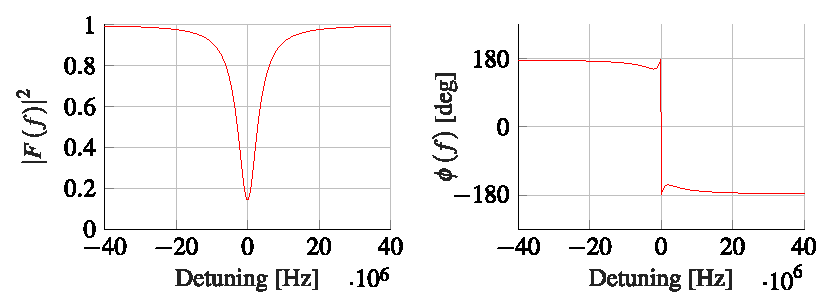
\includegraphics[width=0.9\linewidth]{images/fomega.eps}
	\caption{Module and phase of the field reflected from a Fabry-Perot cavity, while the module is symmetric with the detuning of the incident field, the phase is asymmetric and can thus be used as an error signal.}
	\label{fig:fomega}
\end{figure}

We cannot directly measure the phase of the field with a photodetector, but this is where the PDH technique comes into play: consider a phase modulator, such as an electro-optic modulator, constructed with a nonlinear crystal able to rapidly modulate its refractive index in relation to an applied voltage. The relevant relation is:
\begin{align}
n(E) = n_e - \frac{1}{2}n_e^3 r_{33}E
\end{align}
where $n_e$ is the extraordinary index of the birefringent crystal, $r_{33}$ the relevant component of the electro-optical tensor and $E$ the applied field. If we apply a sinusoidal voltage $V(t) = Ed = V_0 \sin\Omega t$ to the crystal, the radiation passing through the crystal will be described by:
\begin{align}
	E(t) &=  E_0 \exp[-i\omega t + i\,2\pi\, n(t)\, z/\lambda] =\\
		&= E_0 \exp\left[-i\omega t +i\omega \frac{z}{c}(n_e - \frac{1}{2}n_e^3 r_{33}\frac{V_0}{d}\sin\Omega t) \right]
\end{align}

By defining $\beta = \frac{1}{2}\frac{\omega z}{c}n_e^3\frac{V_0}{d}r_{33}$ and redefining $\tilde E_0 = E_0 \exp(i\omega n_e z/c)$ we get
\begin{align}
E(t) = \tilde E_0 \exp(i\omega t)\exp(i\beta \sin\Omega t)
\end{align}

We can expand this result to first order using the Bessel functions $J_k$, obtaining
\begin{align}
	E(t) &\approx \tilde E_0 [J_0(\beta) + 2 i J_1(\beta) \sin\Omega t]\exp(i\omega t )\\
	&= \tilde E_0 [J_0(\beta)e^{i\omega t} + J_1(\beta)e^{i(\omega+\Omega) t} -J_1(\beta)e^{i(\omega-\Omega) t}]
\end{align}

That is, if a single frequency $\omega$ enters the EOM, three different frequencies compose the radiation coming out of the EOM: the carrier $\omega$ and two sidebands $\omega\pm\Omega$. The expansion holds for small modulation ($\beta < 1$).
If this field enters the cavity, the reflected field will be
\begin{align}
	E(t) = \tilde E_0 [F(\omega)J_0(\beta)e^{i\omega t} + F(\omega+\Omega)J_1(\beta)e^{i(\omega+\Omega) t} -F(\omega-\Omega)J_1(\beta)e^{i(\omega-\Omega) t}]
\end{align}

To find an expression for the optical power, which is what the photodiode measures, we consider that $\Omega \gg \delta\omega$ (sidebands distance from the carrier much larger than the cavity linewidth\footnote{This means that while the carrier frequency is coupled with the cavity, the sidebands are completely reflected.}), that $J_\alpha(\beta)\approx \frac{1}{\Gamma(\alpha+1)}\left(\frac{\beta}{2}\right)^2$ and that $P_c \gg P_s$ (power of the carrier much larger than that of the sidebands), after some algebra we get
\begin{align}
	P_\mathrm{ref} \approx P_c |F(\omega)|^2 -2 P_c\beta\Im{F(\omega)}\sin\Omega t + (2\Omega \,\mathrm{terms})
\end{align}

We can now see that it is possible to measure $\Im{F(\omega)}$, all is needed is to remove the $\sin\Omega t$ term with a demodulation (using for example a mixer) and then filter out the $2\Omega$ terms with a low-pass filter.

The full PDH error signal, after demodulating and filtering, is
\begin{align}
	\epsilon_\mathrm{PDH} = -\frac{1}{2}P_c\beta \Im{F(\omega)F^*(\omega+\Omega)-F^*(\omega)F(\omega-\Omega)}
\end{align}
represented in Fig \ref{fig:errsignal}.
Near resonance the error signal has a ``linear zone'': in fact in this case we can write
\begin{align}
	\omega = 2\pi N \nu_\mathrm{FSR} + \delta\omega
\end{align}
where $\delta\omega$ is the detuning from resonance, and from this we get
\begin{align}
	F(\delta\omega) \approx \frac{i}{\pi}\frac{\delta\omega}{\delta\nu}
\end{align}
where $\delta\nu$ is the cavity linewidth. The error signal near resonance then becomes
\begin{align}
	\epsilon_\mathrm{PDH} \approx -\frac{2}{\pi}P_c \beta \frac{\delta\omega}{\delta\nu}
\end{align}
where it is clear its linear dependence from $\delta\omega$. This approximation holds for high finesse caivities and for $\delta\omega \ll \delta\nu$.

\begin{figure}
	\centering
	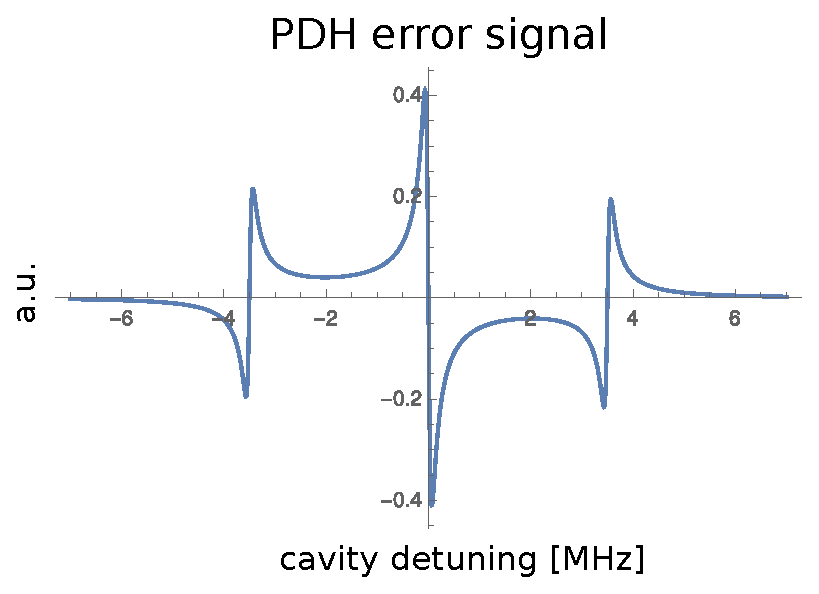
\includegraphics[width=0.8\linewidth]{images/errsignal.eps}
	\caption{The typical PDH error signal. The carrier-sidebands distance is 3.5\,MHz as in our experimental setup. The linear zone can be seen in the center.}
	\label{fig:errsignal}
\end{figure}

\section{Feedback system}

We have seen that the PDH stabilization technique is based on a feedback loop, we now wish to study the stability properties of this loop.

The system can be divided in 5 parts:
\begin{enumerate}
	\item A reference: in our case the mode-locked laser
	\item A source: the Fabry-Perot cavity
	\item A discriminator: the electronic system that generates the error signal, composed by a EOM, a detector, a phase shifter, a mixer and a low-pass filter
	\item A servo: the PID that uses the error signal to drive the piezo
	\item An actuator: the piezo that moves the mirror inside the cavity.
\end{enumerate}
\begin{figure}
	\centering
	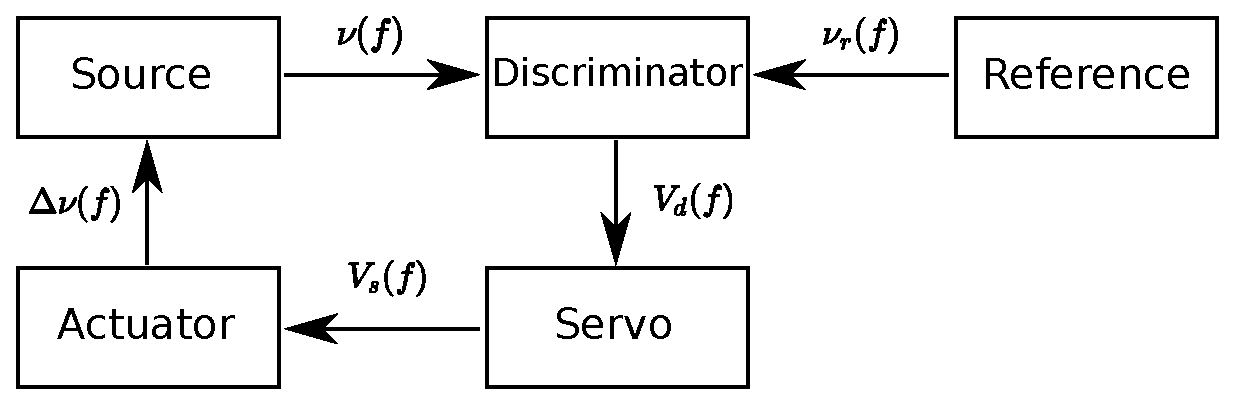
\includegraphics[width=0.9\linewidth]{images/loop.eps}
	\caption{The stabilization system feedback loop.}
	\label{fig:loop}
\end{figure}

The feedback loop is showed in Fig \ref{fig:loop}.

\subsubsection{Discriminator}
Let's consider the frequency signal generated by the reference $\tilde \nu_r(t)$ and that of the source $\tilde \nu(t)$, the purpose of the feedback loop it to minimize $\Delta\tilde\nu = |\tilde\nu_r(t)-\tilde\nu(t)|$. In the Fourier domain the signals are $\nu(f)$ and $\nu_r(f)$, these signals are combined by the discriminator, which outputs a voltage proportional to their difference, that is
\begin{align}
	V_D = D(f) (\nu(f)-\nu_r(f))
\end{align}
where $D(f)$ is the frequency response. From Fig \ref{fig:errsignal} we can see that the frequency response is essentially a constant, the slope of the linear zone $k_d$, multiplied by  the 6th-order Butterworth filter response. The typical Butterworth filter response is shown in Fig \ref{fig:servo}, while the $k_d$ constant can be measured from the error signal during a scan, if $2\Omega =7$\,MHz is the frequency distance between the sidebands, $\Delta t$ their temporal separation during a scan, $\delta V/\delta t$ the difference quotient of two points in the linear zone:
\begin{align}
	k_d = \frac{\delta t}{\delta V} \frac{2\Omega}{\Delta t}
\end{align}

\subsubsection{Servo}
The servo elaborates the error signal and outputs the right voltage to the piezo.
After passing through the servo, the voltage signal becomes
\begin{align}
	V_s = S(f) V_d = S(f)D(f)(\nu(f)-\nu_r(f))
\end{align}
\begin{sidewaysfigure}
	\centering
	\includegraphics[width=0.9\linewidth]{images/pidscheme.pdf}
	\caption{The servo PID circuit.}
	\label{fig:servoscheme}
\end{sidewaysfigure}

where $S(f)$ is the servo PID transfer function. The servo schematic is shown in Fig \ref{fig:servoscheme}: first the error signal goes through an Offset stage, where a DC component can be added to it, then it goes through both the Proportional and Integrator stages, the outputs of which are summed in a summer stage. The signal is then filtered with a single pole LP filter and sent to an amplifier (of fixed gain 3). We must include the piezo actuator response in the circuit: the piezo behaves essentially like a capacitor $C$ in the system, since the PID has output resistance $R$ it constitutes a LP filter with characteristic time $\tau = RC$. All the stages contribute to the frequency response via their transfer functions $G_i$:
\begin{align}
	S(f) = G_\mathrm{offset}(f)[G_\mathrm{int}(f)+G_\mathrm{prop}(f)]G_\mathrm{filter}(f)G_\mathrm{piezo}(f)
\end{align}
where the summer and amplifier stages are considered to have unitary gain (they are composed of Op-Amps in retroactive feedback configuration). The typical servo transfer function is shown in Fig \ref{fig:servo}.
\begin{figure}
	\centering
	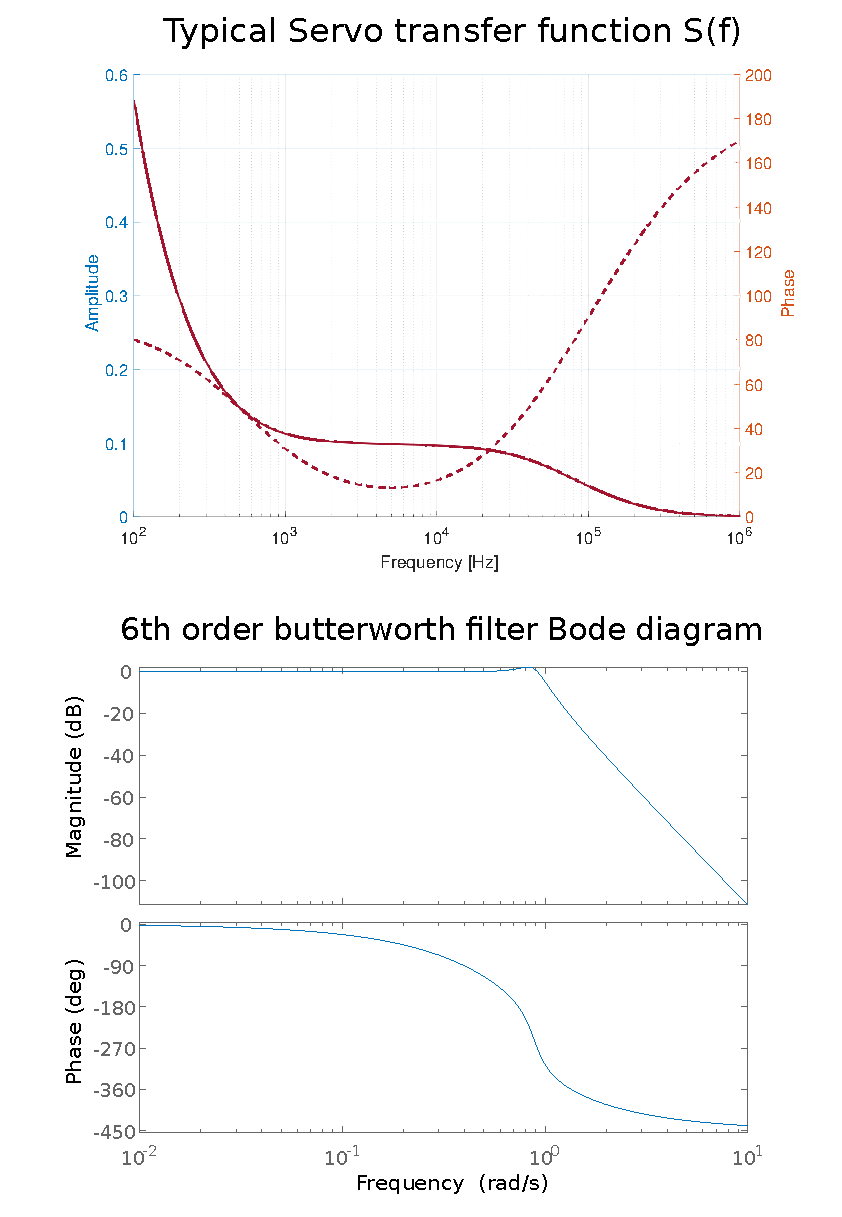
\includegraphics[width=0.8\linewidth]{images/servo.eps}
	\caption{Top: Servo transfer function S(f), the continuous line indicates the amplitude while the dotted one the phase.	Bottom: 6th order Butterworth filter transfer function.}
	\label{fig:servo}
\end{figure}

\subsubsection{Actuator}

The piezo actuator moves the first mirror of the cavity and in doing so converts the voltage signal received by the PID to a frequency signal $\Delta \nu$, that is the change in resonant frequency of the cavity:
\begin{align}
	\Delta \nu(f) = A(f)V_s = A(f)S(f)D(f)(\nu(f)-\nu_r(f))
\end{align}
where $A(f) = k_a \tilde A(f)$ is the piezo transfer function. The piezo, being a moving object, has a frequency response that depends on its mechanical properties and that of its mounting ($\tilde A(f)$), and by acting on the cavity provides a voltage-to-frequency conversion $k_a$. To characterize such a response we built a Michelson interferometer, using the fringes to measure the piezo movement in response to an applied sinusoidal voltage. By choosing the DC component of the sinusoidal voltage in order to place the piezo around the linear part of the fringes, a linear relation between intensity of the fringe and piezo movement can be obtained. Results are shown in Fig \ref{fig:actuator}, the piezo presents a resonance similar to that of an harmonic oscillator near 23000\,Hz. Another part of the transfer function is the voltage-to-frequency conversion ratio $k_a$, this can be measured by observing the transmitted beam. In fact the difference in cavity length between two resonances is $\lambda = 1030\,nm$ and by measuring the change in voltage on the piezo between two peaks the voltage/length relation is found, this can be then converted to a voltage/frequency conversion remembering that $\nu_\mathrm{FSR} = c/L$.
\begin{figure}
	\centering
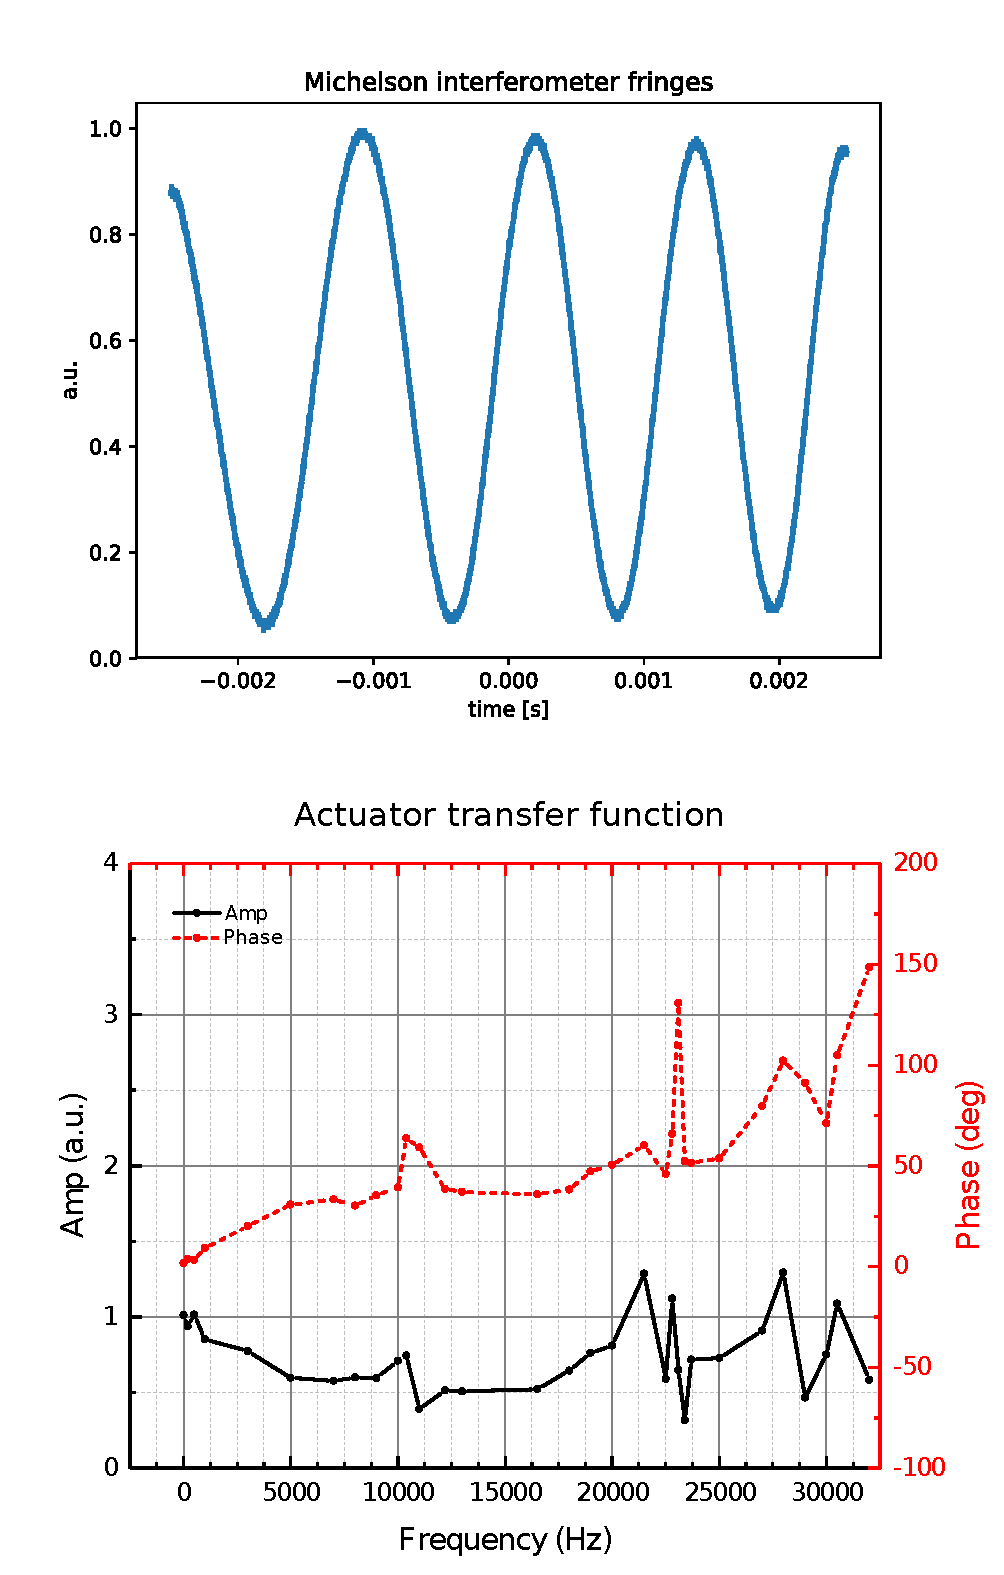
\includegraphics[width=0.8\linewidth]{images/actuator.eps}
\caption{Top: Michelson interference fringes observed by moving the piezo. Around 0.5\,V the movement/intensity relation is linear, so by sending a small sinusoidal voltage we can measure the piezo movements with a photodetector. Bottom: Actuator transfer function measured with the interferometer, for every point a sinusoidal voltage with the desired frequency has been sent to the piezo and the phase and amplitude of the resulting movement recorded.}
\label{fig:actuator}
\end{figure}

\subsubsection{Feedback loop}

The overall transfer function of the system is given by
\begin{align}
	G(f) = A(f)S(f)D(f)
\end{align}
and the actuator changes the resonant frequency of the FP cavity according to (we drop the $f$ dependence):
\begin{align}
	\nu = \nu_0 + ASD(\nu_r-\nu)
\end{align}
where $\nu_0$ is the original cavity frequency. To find the closed loop gain of the system we explicit $\nu$:
\begin{align}
	\nu = \frac{1}{1+G}\nu_0 + \frac{G}{1+G}\nu_r
\end{align}
From this equation we see that to lock the resonant frequency $\nu$ to the reference $\nu_r$ we need the absolute value of G to be as high as possible, in fact in this limit:
\begin{align}
	\frac{1}{1+G} \rightarrow 0 && \frac{G}{1+G} \rightarrow 1
\end{align}
meaning that $\nu=\nu_r$.

We can then calculate how the noises on the source and on the reference (the stochastic processes identified by $\nu(f)$ and $\nu_r(f)$ respectively) are suppressed by the feedback loop, resulting in low relative noise $\Delta\nu(f) = \nu_r(f) -\nu(f)$ between the two. To calculate the power spectral density noise of $\Delta\nu$ we take
\begin{align}
	|\Delta\nu(f)|^2 &= |\nu_r(f) - \nu(f)| ^ 2 =\\
			&= |\nu_r(f)|^2 + |\nu_(f)|^2 -2\Re{\nu(f)\nu_r(f)^*} = \\
			&= |\nu_r(f)|^2 + \left|\frac{1}{1+G(f)}\nu_0(f) + \frac{G(f)}{1+G(f)}\nu_r(f)\right|^2 +\\
			&- 2 \Re{\left(\frac{1}{1+G(f)}\nu_0(f)+\frac{G(f)}{1+G(f)}\nu_r(f)\right)\nu_r(f)^*}
\end{align}

We can assume that the two processes $\nu_r(f)$ and $\nu_0(f)$ are uncorrelated, since they refer to different systems, this means that mixed terms like $\nu_r(f)\nu(f)$ don't contribute, so we can write
\begin{align}
		|\Delta\nu(f)|^2 &= |\nu_r(f)|^2 + \frac{1}{\left|1+G(f)\right|^2}|\nu_0(f)|^2 + \frac{|G(f)|^2}{\left|1+G(f)\right|^2}|\nu_r(f)|^2 +\\ &-2\Re{\frac{G(f)}{1+G(f)}|\nu_r(f)|^2} = \\
		&=\frac{1}{\left|1+G(f)\right|^2}|\nu_0(f)|^2 + \frac{1}{\left|1+G(f)\right|^2}|\nu_r(f)|^2
\end{align}
Writing in terms of the power spectral densities $S_{\Delta\nu}(f)$, $S_{r}(f)$ and $S_{0}(f)$:
\begin{align}
S_{\Delta\nu}(f) = \frac{1}{\left|1+G(f)\right|^2} \left[S_{0}(f) + S_{r}(f)\right]
\end{align}
It is clear that by maximizing the loop gain, in particular by maximizing $\left|1+G(f)\right|^2$, the noise between source and reference is suppressed.

Feedback instabilities can arise when $G(f)=-1$: if this relation is satisfied for some $f$ then the system will oscillate at that frequency. This is the so-called Barkhausen stability criterion: when the phase of the loop gain $G$ is close to $\pi +2n\pi$ its absolute value must be $|G|\ne1$ to avoid auto-oscillations. Satisfying this criterion is the purpose of the LP single pole filter in the servo PID: by regulating the cutoff frequency we can make sure that $|G|<1 $ when $\angle G \approx \pi +2n\pi$.

The stabilization procedure will be explained in the next chapter, where also the  measurements of the Power Spectral Density noise of the stabilized cavities will be presented.

\begin{figure}
	\centering
	\includegraphics[width=0.7\linewidth]{images/foto/actuator.jpg}
	\caption{The mirror A mounting containing the piezo ring actuator.}
	\label{fig:fotoactu}
\end{figure}
\begin{figure}
	\centering
	\includegraphics[width=0.9\linewidth]{images/foto/discr.jpg}
	\caption{The discriminator stage. Left: the photodetector monitoring the blue cavity reflected beam. Right: phase shifters, mixers, and LP filters for both the cavities, the PDH signal is sent from the filters to the servo PID. }
	\label{fig:discr}
\end{figure}
\begin{figure}
	\centering
	\includegraphics[width=0.9\linewidth]{images/foto/pid.png}
	\caption{The servo stages used to drive the piezo in both cavities. }
	\label{fig:pid}
\end{figure}